\documentclass{beamer}
\usepackage{amsfonts,amsmath,oldgerm}
\usepackage[export]{adjustbox}
\usefonttheme[onlymath]{serif}
\usepackage{slashed}
\usetheme{sintef}
\newcommand{\testcolor}[1]{\colorbox{#1}{\textcolor{#1}{test}}~\texttt{#1}}
\newcommand{\la}{\langle}
\newcommand{\ra}{\rangle}
\usefonttheme[onlymath]{serif}

%%%%%% COMMANDS LIST
%\vspace{\baselineskip}

%%%%%% TITLE
\titlebackground*{assets/background}
\newcommand{\hrefcol}[2]{\textcolor{cyan}{\href{#1}{#2}}}
\title{Non-perturbative computation of Kaon oscillation amplitudes in Lattice QCD with $N_f = 2+1$ sea quarks and OBC}
\course{Master's Degree in Theoretical Physics\vspace*{.1mm}}
\author{{\rm Supervisor: Prof.} Mauro Papinutto \\ \href{mailto:emanuele.rosi@roma1.infn.it}{Emanuele Rosi}}
\IDnumber{1812180}
\date{Academic Year 2022/2023}

%%%%%% DOCUMENT
\begin{document}
\maketitle

\section{Introduction to $K^0$-$\bar K^0$ mixing}

\begin{frame}{Kaon oscillations}
      \framesubtitle{SM oscillations}
      Kaon oscillations in Standard Model (SM) are mediated by Weak Interactions.
      \begin{itemize}
            \item Two 1-loop order diagrams
      \end{itemize}
      \vspace{\baselineskip}
      \begin{columns}
            \centering
            \begin{column}{0.5\textwidth}
                  \centering
                  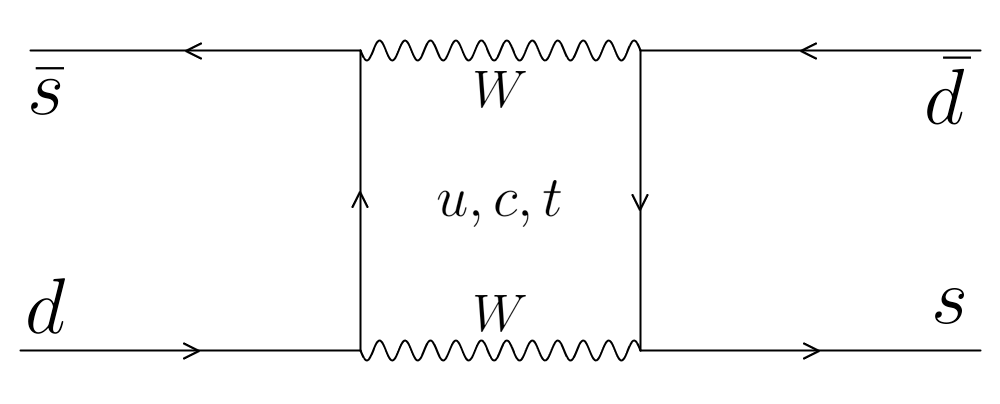
\includegraphics[width=.8\textwidth,right]{assets/kkbar-1.png}
            \end{column}
            \begin{column}{0.5\textwidth}
                  \centering
                  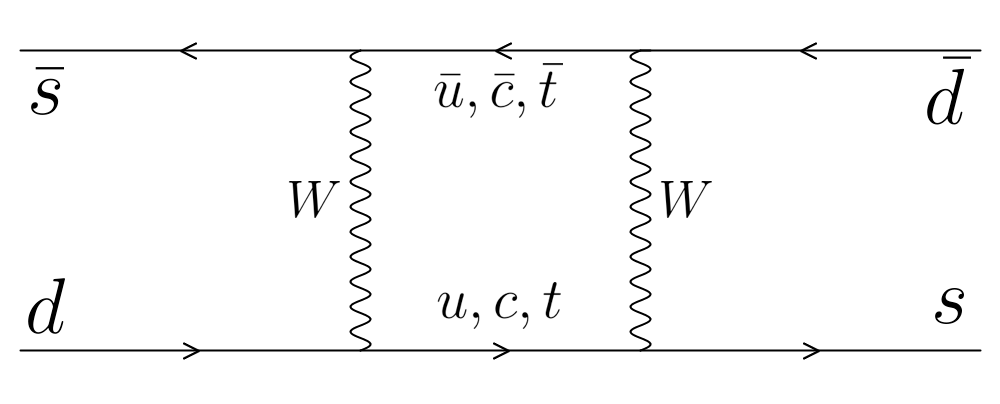
\includegraphics[width=.8\textwidth,left]{assets/kkbar-2.png}
            \end{column}
      \end{columns}
\end{frame}

\begin{frame}{Kaons oscillations}
      \framesubtitle{SM oscillations}
      Kaons oscillations in Standard Model (SM) are mediated by Weak Interactions.
      \begin{itemize}
            \item Two 1-loop order diagrams
            \item Effective mixing operator ($E \ll M_W$):
            \begin{equation*}
                  \la \bar K^0 | \Theta_1 | K^0 \ra \qquad \Theta_1 = \Big[ \bar s^a \gamma_\mu (1-\gamma_5) d^a \Big] \cdot \Big[ \bar s^b \gamma_\mu (1-\gamma_5) d^b \Big]
            \end{equation*}
            \item $B_1$ parameter parametrizes deviation from the Vacuum Insertion Approximation (VIA):
            \begin{equation*}
                  \la \bar K^0 | \Theta_1 | K^0 \ra = B_1 \la \bar K^0 | \Theta_1 | K^0 \ra_\text{VIA} = \frac{8}{3} B_1 F_K^2 m_K^2
            \end{equation*}
      \end{itemize}
\end{frame}

\begin{frame}[fragile]{Kaon oscillations}
      \framesubtitle{Oscillations BSM}
      \begin{itemize}
            \item $B_1$ parameter (a.k.a. $B_K$) parametrizes deviation from VIA
            \item Other operators $\{\Theta_i,\tilde\Theta_j\}$ appear in theories beyond the SM (BSM) $[5]$
            \item They form a complete set of {\bf operators of dimension 6 - composed by 4 quarks}, closed under renormalization procedure
            \item Definition of \emph{bag parameters} $B_j$ $[1]$:
            \begin{equation*}
                  \la \bar K^0 | \Theta_j^{[+],\text{ren}} (\mu) | K^0 \ra = \xi_j \left(\frac{m_K^2}{m_s(\mu)+m_d(\mu)}\right)^2 f_K^2 B_j(\mu) \qquad j \ge 2
            \end{equation*}
      \end{itemize}
\end{frame}

\begin{frame}{Purpose of the work}
      \framesubtitle{Introduction}
      \centering
      Non perturbative computation of bare bag parameters $B_i$
      $$\downarrow$$
      Path integral formalism - lattice QCD
      $$\downarrow$$
      Coordinated Lattice Simulations (CLS) gauge configurations with $N_f = 2+1 $\\ sea quarks and open boundary conditions (OBC) in time direction
\end{frame}

\section{Quantum Field Theories on the Lattice}

\begin{frame}{Lattice regularizations of QFTs}
      Regularizations ingredients:
      \begin{itemize}
            \item Finite lattice space $\Lambda$: $L \times L \times L \times T$
            \item Lattice spacing $a$: $L = a\cdot N_L$, $T = a\cdot N_T$
            \item Action discretization:
            \begin{equation*}
                  S^\text{lat}[a;\tilde\phi_1,\dots,\tilde\phi_{N_\text{fields}}] \hspace*{1mm} \xrightarrow{\hspace*{3mm} a \rightarrow 0\hspace*{3mm}} \hspace*{1mm} S^\text{cont}[\phi_1,\dots,\phi_{N_\text{fields}}]
            \end{equation*}
            \item $O(a^n)$-improvement:  $S^\text{lat}(a) = S^\text{cont} + o(a^{n})$
            \item Troubles: finite volume effects \& lattice spacing effects
      \end{itemize}
\end{frame}

\begin{frame}{Sea vs Valence quarks}
      \begin{columns}
            \begin{column}{0.5\textwidth}
                  \begin{itemize}
                        \item Sea and valence quarks are regularized through different actions
                        \begin{center}
                              $\downarrow$\\Theoretical advantages in lattice QCD
                        \end{center}
                        \item Sea sector: $N_f = 2+1$ quarks + gluons\\Valence sector: $d,s$ quarks
                  \end{itemize}
            \end{column}
            \begin{column}{0.45\textwidth}
                  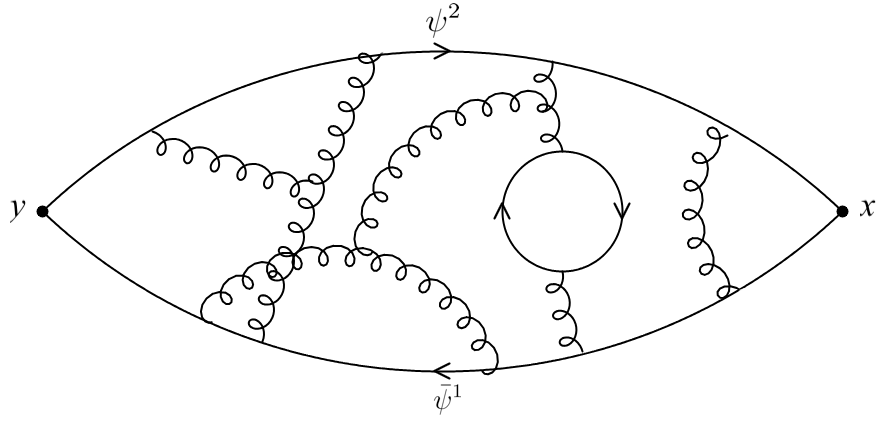
\includegraphics[width=\textwidth]{assets/confinement_bis.png}
                  $$G^{12}(x,y) = \left\la M(x)\overline M(y) \right\ra$$
            \end{column}
      \end{columns}
\end{frame}

\begin{frame}{Sea sector}
      \begin{itemize}%[<+->]
            \item Gauge configuration exhibit {\bf long autocorrelation times} as $a\rightarrow 0$
            \item Zero modes of Dirac Wilson operator $D^W$ make the sea quarks simulation inefficient 
            \item[]\begin{center}
                  $\Downarrow$\\
                  {\bf Open boundary conditions (OBC) in time direction} $[4]$
                  \end{center}\vspace{\baselineskip}
            %% \item Restoration of connection of gauge fields space
            %% \\IR protection against null eigenvalues of $D^W$
            \item Gauge fields: Luscher-Weisz action
            \item Sea quarks: Dirac-Wilson action + Sheikholeslami-Wohlert term ($O(a)$-improved)
      \end{itemize}
\end{frame}

\begin{frame}{Valence sector}
      \begin{itemize}
            \item Valence quarks: Osterwalder-Seiler at Maximal twist + SW term
            \item Flavours: $d,d',s,s'$ with different signs Wilson parameters $r_i$
            \\ $\Longrightarrow$ R. Frezzotti \& G. Rossi strategy $[3]$
      \end{itemize}
      \vspace{\baselineskip}
      {\bf Achievements:}
      \begin{itemize}%[<+->]
            \item $O(a)$-improved mixing amplitudes w/o the need for W.A.
            \item Absence of wrong chirality mixing between $\{O_i^{[+]}\}$ and $\{O_i^{[-]}\}$
            \item Blocks like renormalization matrix $[Z_{ij}]$ for parity odd operators $[2]$
      \end{itemize}
\end{frame}

\section{Bag parameters extrapolation}

\begin{frame}{Bag parameters extrapolation}
      \begin{columns}
            \begin{column}{0.5\textwidth}
                  \begin{equation*}
                        \begin{split}
                              & C_i (x_4,y_4,z_4) = \sum_{\vec x,\vec y,\vec z}     \la \bar K^{0'}(x)O_{i[+]}(y)\bar K^{0} (z) \ra  \\
                              & G_{34} (x_4,y_4) = \sum_{\vec x,\vec y}             \la \bar K^{0'} (x) K^{0'} (y)              \ra \\
                              & G_{12} (x_4,y_4) = \sum_{\vec x,\vec y}             \la \bar K^{0} (x) K^{0} (y)                \ra \\
                              & X_{34} (x_4,y_4) = \sum_{\vec x,\vec y}             \la      A_{4}' (x) K^{0'} (y)              \ra \\
                              & X_{12} (x_4,y_4) = \sum_{\vec x,\vec y}             \la      A_{4} (x) K^{0} (y)                \ra \\          
                        \end{split}
                  \end{equation*}
            \end{column}
            \begin{column}{0.5\textwidth}
                  \begin{center}
                        Path integral allows to calculate only VEVs$$\la 0 | \cdots | 0 \ra$$
                        $$\downarrow$$
                        Method based on asymptotic behaviours for large euclidean time separations
                  \end{center}
            \end{column}
      \end{columns}
\end{frame}

\begin{frame}{Bag parameters extrapolation}
      Bag parameters are recovered in continuum limit $a \rightarrow 0$ for $x_4 \gg y_4 \gg z_4$:
      \begin{equation*}
            \begin{split}
                  & \mathcal{B}_1 (a) \approx \frac{3}{8}\cdot\frac{C_1(x_4,y_4,z_4)}{X_{34}(x_4,y_4)X_{12}(y_4,z_4)} \xrightarrow{ \quad a \rightarrow 0 \quad } B_K \\
                  & \mathcal{B}_i (a) \approx \frac{1}{\xi_i}\cdot\frac{\Lambda_{ij}C_j(x_4,y_4,z_4)}{G_{34}(x_4,y_4)G_{12}(y_4,z_4)} \xrightarrow{ \quad a \rightarrow 0 \quad } B_i \\
                  & \mathcal{R}_i (a) \approx \Lambda_{ij}\cdot\frac{C_j(x_4,y_4,z_4)}{C_1(x_4,y_4,z_4)}\xrightarrow{ \quad a \rightarrow 0 \quad } R_i = \frac{B_i}{B_K} \\
            \end{split}
      \end{equation*}
      $\Rightarrow$ Need for 2 and 3 points integrated correlation functions computation
\end{frame}

\section{Simulation Program}

\begin{frame}{Noise spinors method}
      \begin{columns}
            \begin{column}{0.65\textwidth}
                  Mesonic sources in $x_4$ and $z_4$ are simulated through noise spinors $\eta^{(x_4)}$ and $\eta^{(z_4)}$:
                  \begin{itemize}%[<+->]
                        \item Two sets of $N_n$ spinors randomly generated
                        \item The sums $\sum_{\vec{x}}$ and $\sum_{\vec{z}}$ automatically implied when calculating the average over $\eta$s
                        \item Computational advantage
                        \item Different Wick contractions are obtained by multiplying propagators from sources with Dirac matrices
                  \end{itemize}
            \end{column}
            \begin{column}{0.35\textwidth}
                  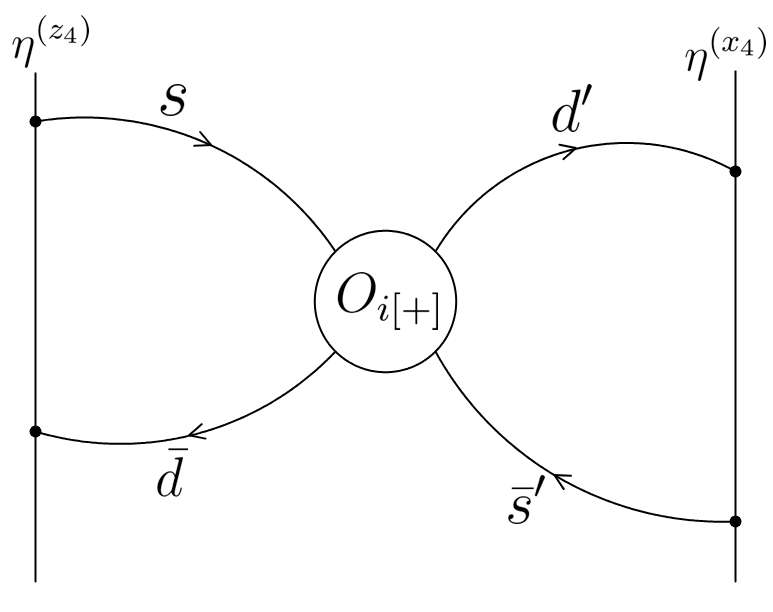
\includegraphics[width=\textwidth]{assets/eta-spinors.png}
            \end{column}
      \end{columns}
\end{frame}

\begin{frame}{Simulation program tests}
      Tests:
      \begin{itemize}
            \item Gauge invariance test
            \item Gauge invariance test + investigation about $N_n$
            \item Test on \emph{Tree level improved Symanzik action}, quenched approximation
            \item Test on \emph{Plaquette gauge action}, quenched approximation
      \end{itemize}
\end{frame}

\begin{frame}{Test \#1: Gauge invariance}
      Gauge transformed propagators:\newline
      \begin{equation*}
            \left(S^{(f)}(y, x)[\Omega U \Omega^\dagger]\right)^{b,a}_{\beta,\alpha} = \Omega (y)^{b,c} \left(S^{(f)}(y,x)[U]\right)^{c,d}_{\beta,\alpha} \Omega^\dagger (x)^{d,a}
      \end{equation*}
      \begin{itemize}
            \item Equation tested in three points integrated correlators $C_{i,[+]}$
            \item Link variables $U_\mu (x)$ are randomly generated and then transformed
            \item Pointlike sources instead of random spinors $\eta$
      \end{itemize}
      \begin{equation*}
            \begin{gathered}
                  \text{Relative errors: } \varepsilon_i \lesssim 10^{-13} \\
                  \text{Mean relative error: } \bar \varepsilon = (1.313 \pm 1.634) \cdot 10^{-13}
            \end{gathered}
      \end{equation*}
\end{frame}

\begin{frame}{Test \#2: Gauge invariance and investigation about $N_n$}
      \begin{columns}
            \begin{column}{0.43\textwidth}
                  \begin{itemize}
                        \item Equation tested in three points integrated correlators $C_{i,[+]}$
                        \item Link variables $U_\mu (x)$ are randomly generated and then transformed
                        \item Use of random spinors $\eta$
                        \item Different number of $N_n$ were tested. Estimator:
                        \begin{equation*}
                              \varepsilon(N_n) = \frac{1}{N_T-2}\sum_{y_4}\left(\frac{|C(y_4)-\tilde C(y_4)|}{C(y_4)+\tilde C(y_4)}\right)
                        \end{equation*}
                  \end{itemize}
            \end{column}
            \begin{column}{0.57\textwidth}
                  \begin{center}
                        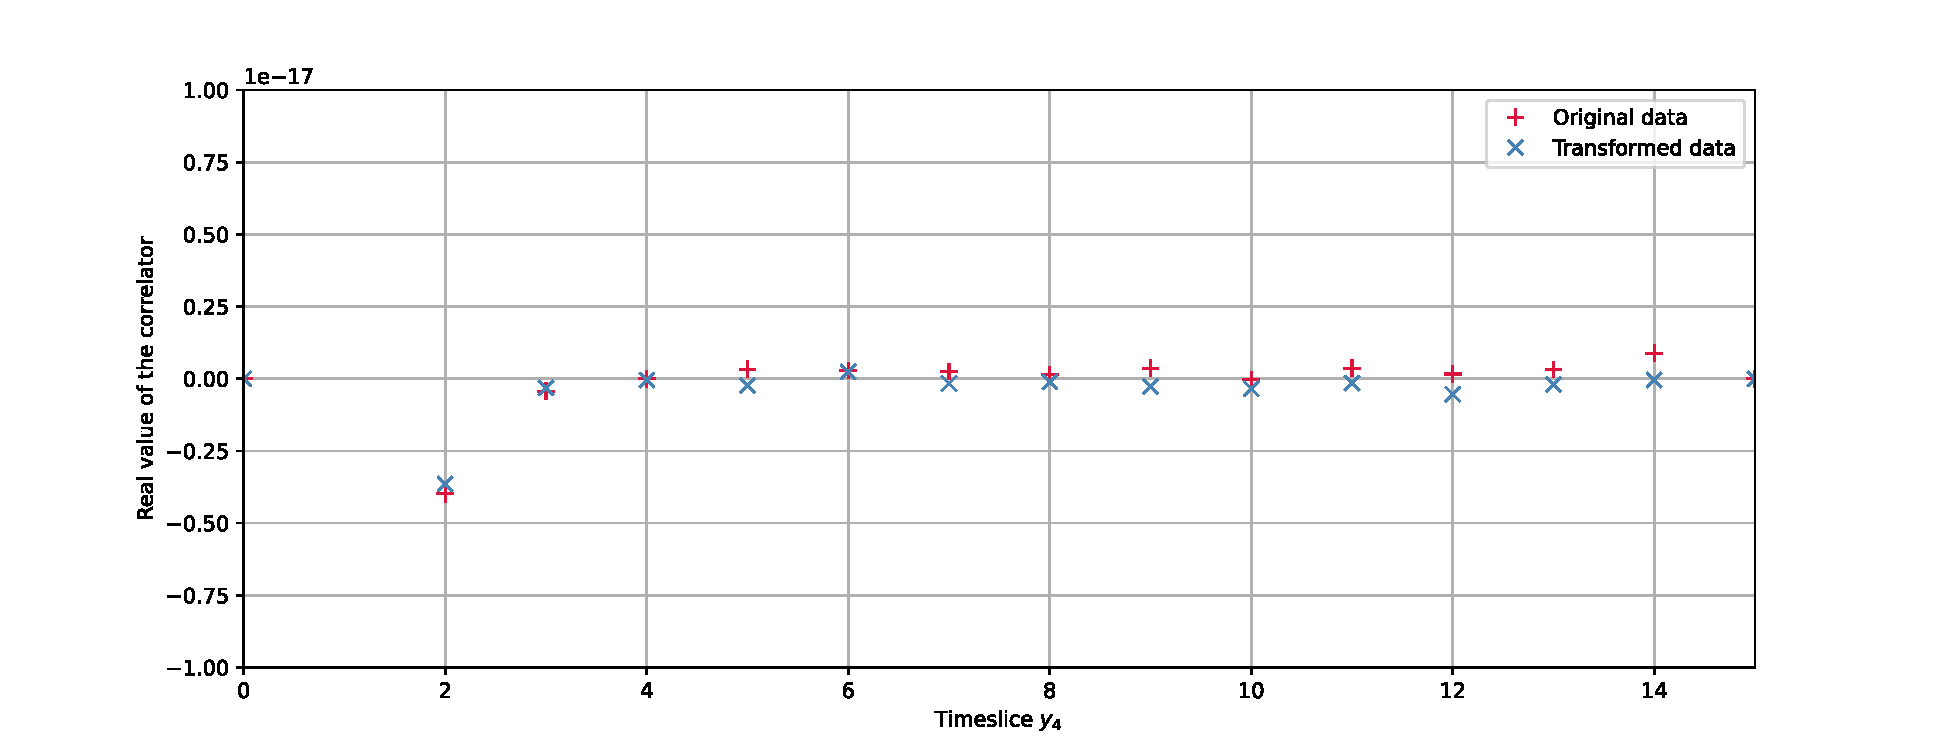
\includegraphics[width=.8\textwidth]{../thesis-tex/imgs-MSc-thesis/check2-20.pdf}\\
                        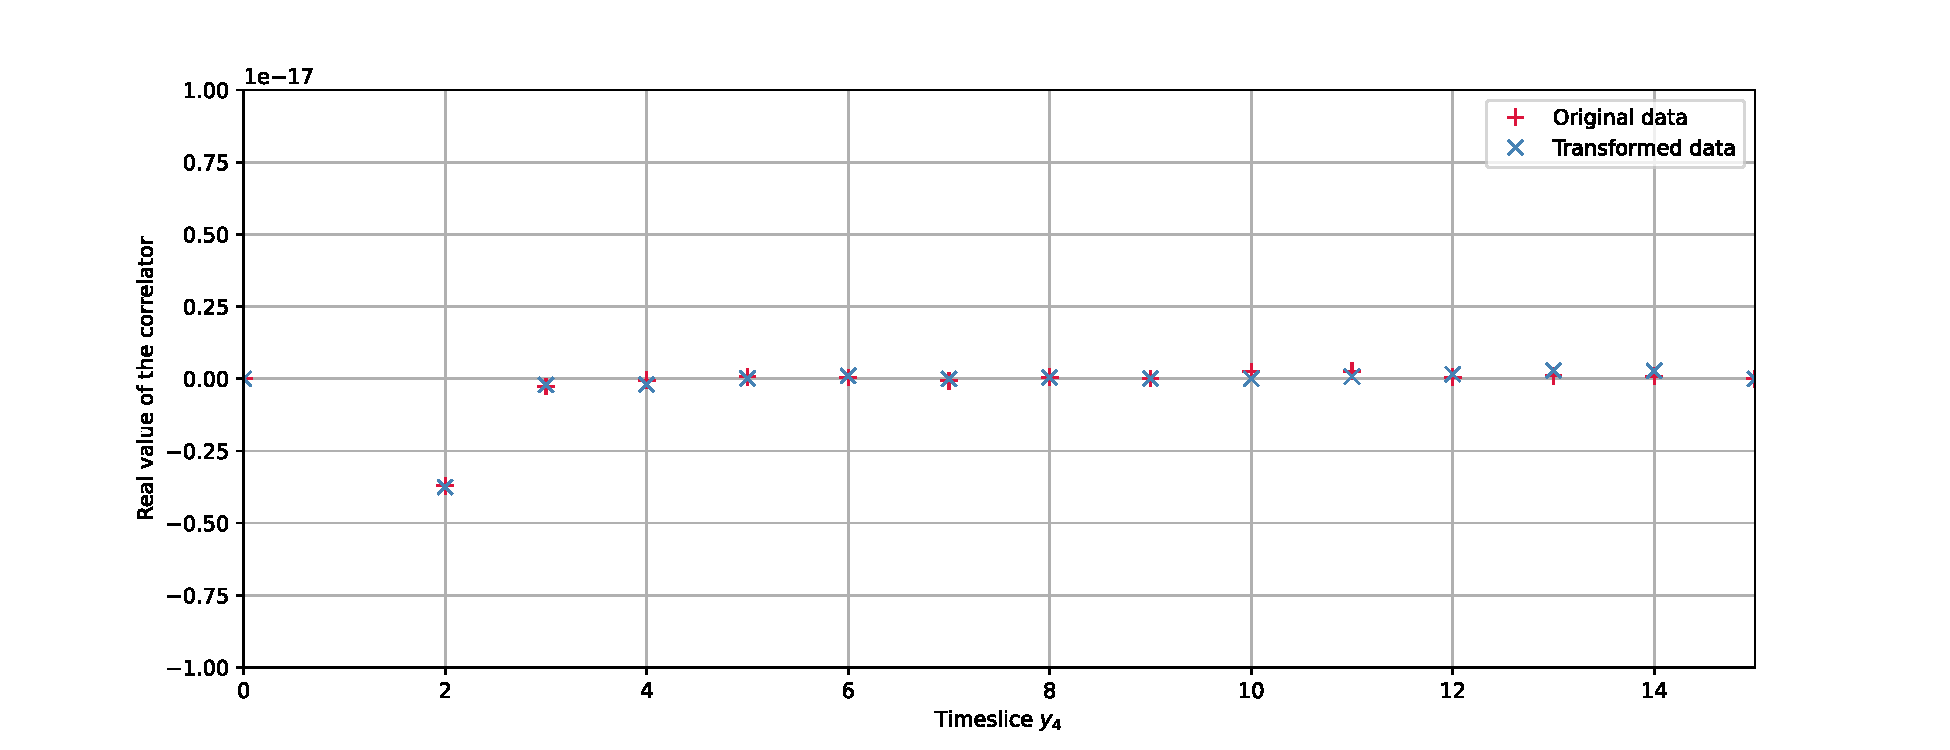
\includegraphics[width=.8\textwidth]{../thesis-tex/imgs-MSc-thesis/check2-100.pdf}
                  \end{center}
            \end{column}
      \end{columns}
\end{frame}

\begin{frame}{Test \#3: tree level improved Symanzik}
      54 Gauge configurations - tree level improved Symanzik action\newline
      16x16x16x32 lattice, $\beta = 6.0$, OBCs, unphysical parameters.
      \begin{columns}
            \begin{column}{.5\textwidth}
                  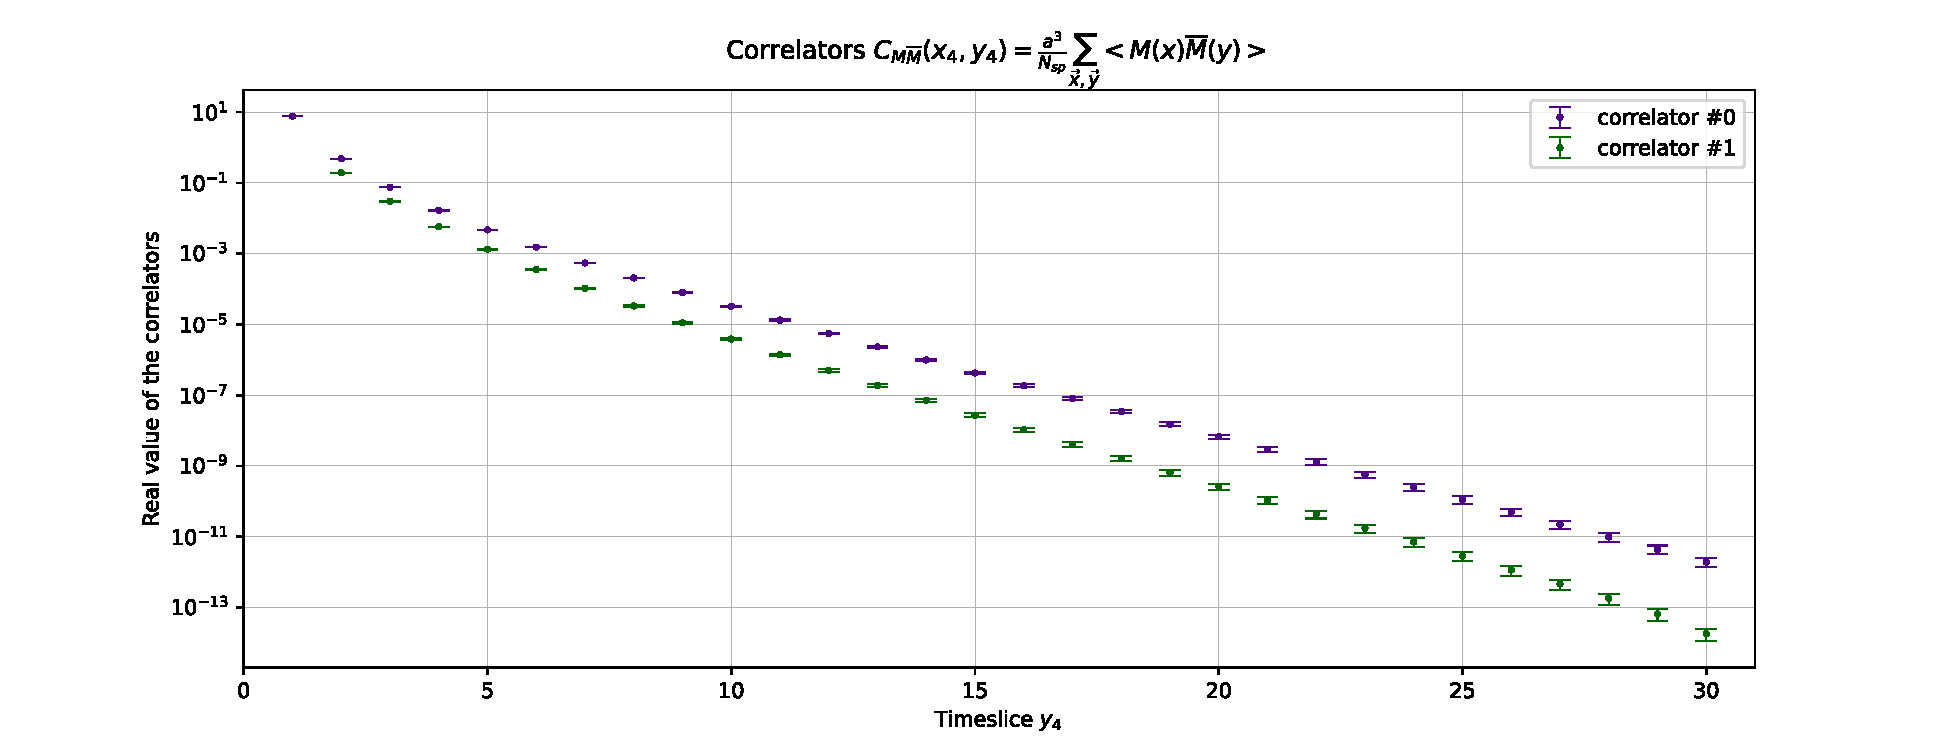
\includegraphics[width=\textwidth]{../thesis-tex/imgs-MSc-thesis/pureYM-2pts.pdf}
                  $$G_{12}(x_4,a), G_{34}(x_4,a)$$
            \end{column}
            \begin{column}{.5\textwidth}
                  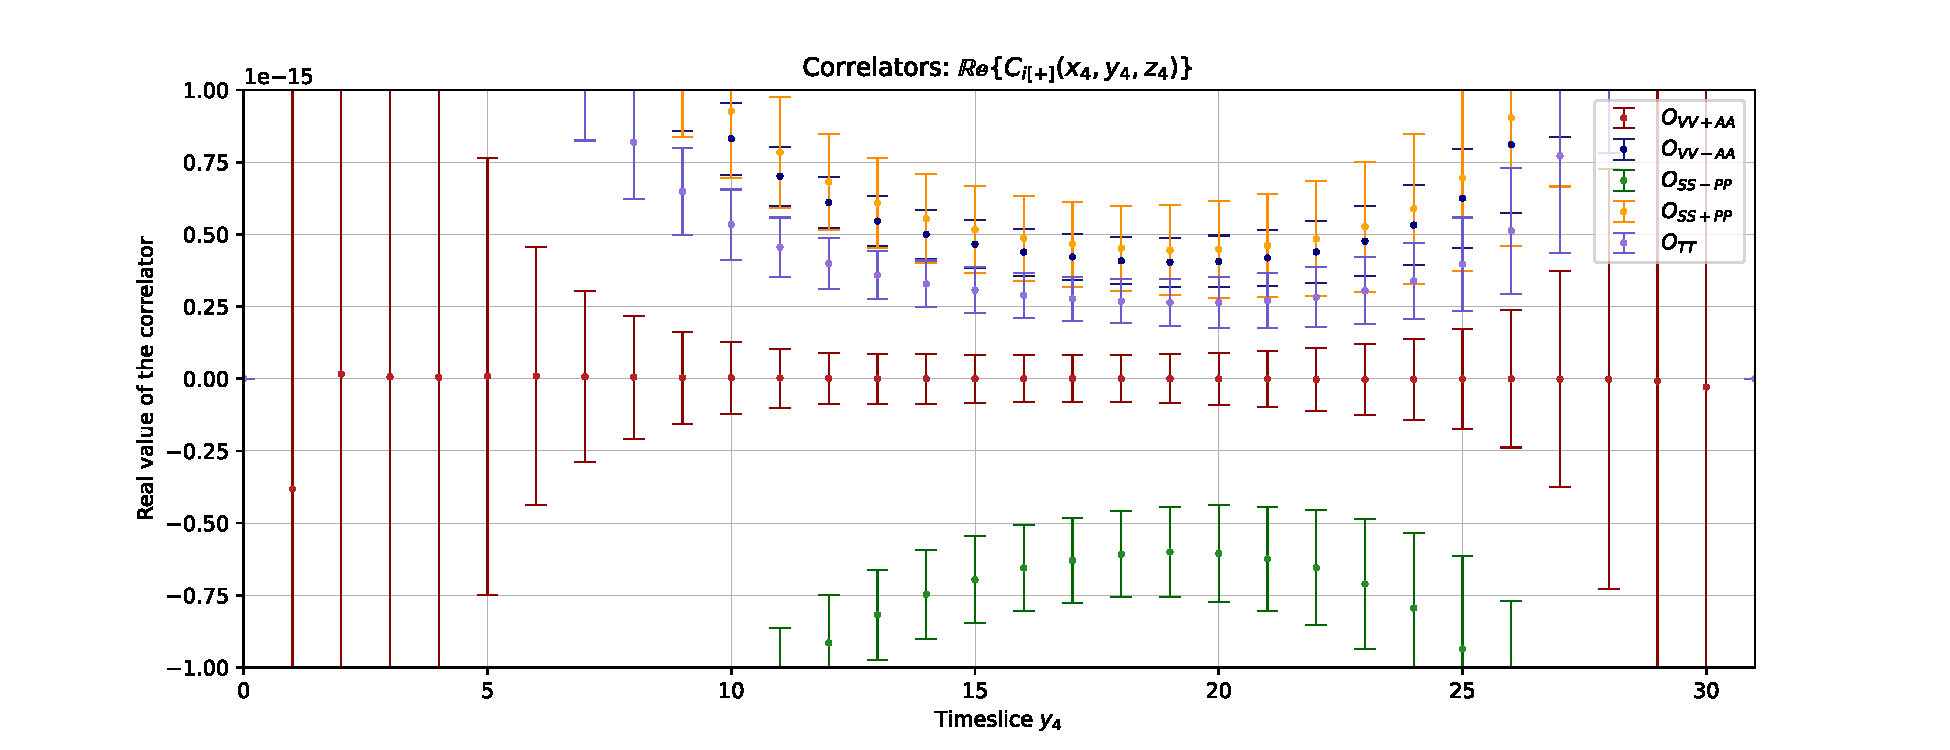
\includegraphics[width=\textwidth]{../thesis-tex/imgs-MSc-thesis/pureYM-3pts.pdf}
                  $$C_{i[+]}(14a,y_4,a)$$
            \end{column}
      \end{columns}
\end{frame}

\begin{frame}{Test \#4: Plaquette gauge action}
      37 Gauge configurations - plaquette gauge action\newline
      16x16x16x32 lattice, $\beta = 6.0$, OBCs, maximal twist achieved
      \begin{columns}
            \begin{column}{.5\textwidth}
                  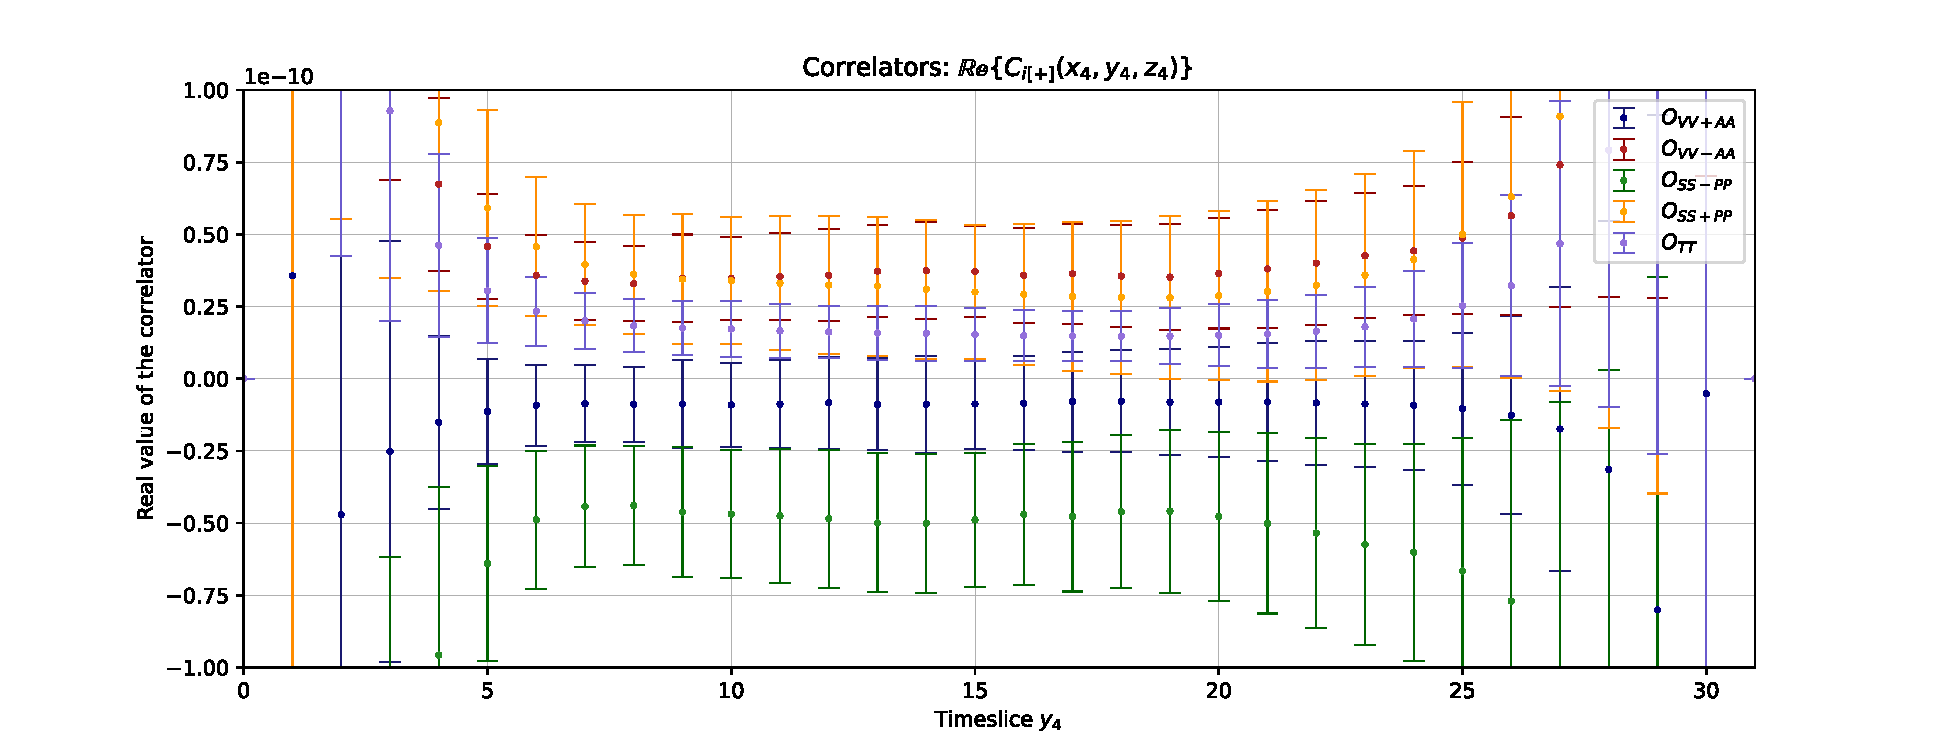
\includegraphics[width=\textwidth]{../thesis-tex/imgs-MSc-thesis/plaq-3pts.pdf}
                  $$C_{i[+]}(14a,y_4,a)$$
            \end{column}
            \begin{column}{.5\textwidth}
                  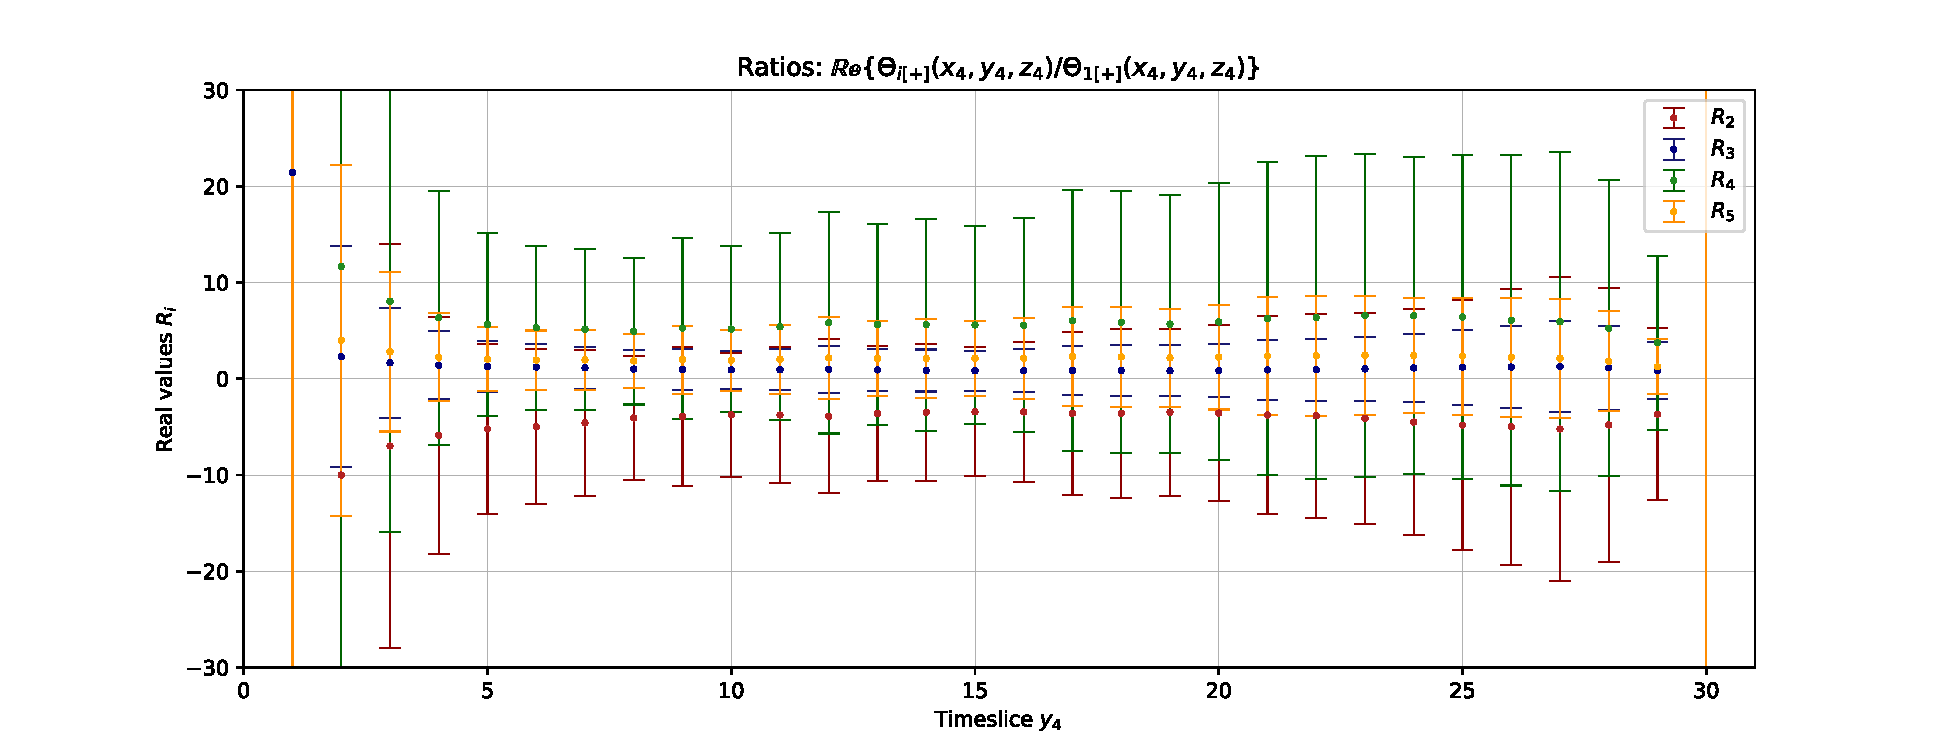
\includegraphics[width=\textwidth]{../thesis-tex/imgs-MSc-thesis/ratios.pdf}
                  $$\mathcal{R}_i (14a,y_4,a) = \Lambda_{ij}\frac{C_{i[+]}(14a,y_4,a)}{C_{1[+]}(14a,y_4,a)}$$
            \end{column}
      \end{columns}
\end{frame}

\begin{frame}{Future developments}
      \begin{itemize}
            \item Numerical simulations with the $N_f = 2+1$ CLS sea ensembles
            \item Data analysis 
            \item Renormalization procedure $[2]$
            \item Continuum limit extrapolation of $B_i$ and $R_i$
            \item Comparison with other lattice results $[6]$
      \end{itemize}
\end{frame}

\begin{frame}[noframenumbering]{Bibliography}
      \framesubtitle{\hspace*{1pt}}
      \begin{enumerate}
            \item V. Bertone et al. ``Kaon mixing beyond the SM from $N_f = 2$ tmQCD and model independent constraints from the UTA''. In: Journal of High Energy Physics 2013.3
            \item Dimopoulos, P., Herdoiza, G., Papinutto, M. et al. ``Non-perturbative renormalisation and running of BSM four-quark operators in $N_f = 2$ QCD.'' Eur. Phys. J. C 78, 579
            \item R Frezzotti and G.C Rossi. ``Chirally improving Wilson fermions II. Four quark operators''. In: Journal of High Energy Physics 2004.10
            \item M. Luscher and S. Schaefer. ``Lattice QCD with open boundary conditions and twisted mass reweighting''. In: Computer Physics Communications 184.3
            \item C.R. Allton et al. ``B-parameters for $\Delta$S = 2 supersymmetric operators''. In: Physics Letters B 453.1-2
            \item S. Aoki et al., ``FLAG Review 2021''. In: The European Physical Journal C 82.10
      \end{enumerate}
\end{frame}

\begin{chapter}[assets/background_negative]{}{\emph{Thank you for listening!}}
      \framesubtitle{\hspace*{1pt}}
\end{chapter}

\begin{frame}[noframenumbering]{$\star$ Action regularizations}
      \framesubtitle{\hspace*{1pt}}
      Many regularizations have been developed
      \vspace{\baselineskip}
      \begin{columns}
            \begin{column}{0.45\textwidth}
                  Gauge actions:
                  \begin{itemize}
                        \item Link variables $$U_\mu (x) = \text{exp}\left(i\int_x^{x+a\hat\mu} A_\nu(\omega)d\omega^\nu \right)$$
                        \item Wilson loops are gauge invariant 
                        \item Plaquette, tree level improved Symanzik, Luscher Weisz
                  \end{itemize}
            \end{column}
            \begin{column}{0.45\textwidth}
                  Fermion actions:
                  \begin{itemize}
                        \item Wilson-Dirac action\\Wilson term $r \in [-1,1]$
                        \item Sheikholeslami-Wohlert term: $$ D^W_{xy} \longmapsto D^W_{xy} + c_{SW} \frac{ia}{4}\sigma_{\mu\nu}\hat F_{\mu\nu} (x) \delta_{xy} $$
                        \item Osterwalder-Seiler action\\(twist transformation)
                  \end{itemize}
            \end{column}
      \end{columns}
\end{frame}

\begin{frame}[noframenumbering]{$\star$ Sea sector}
      \framesubtitle{\hspace*{1pt}}
      \begin{itemize}%[<+->]
            \item Gauge action: Luscher-Weisz action
            $$ S_G[U] = \frac{1}{g_0^2}\left(\frac{5}{3}\sum_{\{P\}} \text{Tr}\left(\mathbb{I} - U_P \right) - \frac{1}{12}\sum_{\{R\}}\text{Tr}\left( \mathbb{I}-U_R \right) \right)$$
            \item Sea quarks: Dirac-Wilson + SW term
            $$ S^\text{sea}[U,f,\bar f] = \sum_{q=1}^3 \sum_{x} \bar f_q (x) \left[ D^{WD}(r_q) + \frac{ia}{4}c_{SW}\sigma_{\mu\nu}\hat{F}_{\mu\nu} + m^\text{bare}_q \right] f_q (x) $$
      \end{itemize}
\end{frame}

\begin{frame}[noframenumbering]{$\star$ Valence sector}{Frezzotti \& Rossi Strategy: an overview $\star$}
      \framesubtitle{\hspace*{1pt}}
      \begin{center}
            Operators $\{\Theta_i^{[\pm]}\}$ in continuum QCD $\xrightarrow{ \text{basis change} }$ Operators $\{Q_i^{[\pm]}\}$ in continuum QCD\\
            \vspace{\baselineskip}
            $\xrightarrow{ \text{flavour replicas} }$ P.E. operators $\{O_{i,[+]}^\text{phys}\}$ $\xrightarrow{ \text{maximal twist} }$ P.E. operators $\{O_{i,[+]}^\text{tw}\}$
      \end{center}
      \vspace{\baselineskip}
      Flavour replicas and twist - an example $\left[\chi^j = \text{physical } \big| \psi^j = \text{twisted}\right]$
      \begin{equation*}
            \begin{split}
                  & \bar{K}^{0'}=\bar s' \gamma_5 d' = \bar \chi^3 \gamma_5 \chi^4 \\
                  & \bar{K}^{0} =\bar s\gamma_5 d = \bar \chi^1 \gamma_5 \chi^2
            \end{split}
            \quad \text{Maximal Twist } \chi^i = e^{i\gamma_5 r_i \frac{\pi}{4}}\psi^i \qquad
            \begin{split}
                  & \bar{K}^{0'}=\bar \psi^3 \gamma_5 \psi^4 \\
                  & \bar{K}^{0} = i \bar \psi^1 \psi^2
            \end{split}
      \end{equation*}
      Similar transformations act on operators $O_{i[+]}$ and map PE operators in PO ones.
\end{frame}

\begin{frame}[noframenumbering]{$\star$ Asymptotic behaviours}
      \framesubtitle{\hspace*{1pt}}
      Asymptotic behaviours for $x_4 \gg y_4 \gg z_4$:
      \begin{equation*}
            \begin{split}
                  & C_i (x_4,y_4,z_4) \approx \sum_{\vec{y}} \la \Omega | \bar K^{0'} | \bar K^{0'} \ra \la \bar K^{0'} | O_{i[+]} | K^{0} \ra \la K^{0} | \bar K^{0} | \Omega \ra e^{-m_{K'} (x_4-y_4)-m_K (y_4-z_4)}\\
                  & G_{34} (x_4,y_4)  \approx \sum_{\vec{y}} \la \Omega | \bar K^{0'} | \bar K^{0'} \ra \la \bar K^{0'} | K^{0'}                    | \Omega \ra e^{-m_{K'} (x_4-y_4)} \\
                  & G_{12} (x_4,y_4)  \approx \sum_{\vec{y}} \la \Omega | \bar K^{0}  | \bar K^{0}  \ra \la \bar K^{0}  | K^{0}                     | \Omega \ra e^{-m_K (x_4-y_4)}    \\
                  & X_{34} (x_4,y_4)  \approx \sum_{\vec{y}} \la \Omega |      A_{4}' | \bar K^{0'} \ra \la \bar K^{0'} | K^{0'}                    | \Omega \ra e^{-m_{K'} (x_4-y_4)} \\
                  & X_{12} (x_4,y_4)  \approx \sum_{\vec{y}} \la \Omega |      A_{4}  | \bar K^{0}  \ra \la \bar K^{0}  | K^{0}                     | \Omega \ra e^{-m_K (x_4-y_4)}    \\                  
            \end{split}
      \end{equation*}
\end{frame}

\begin{frame}[noframenumbering]{$\star$ Noise spinors method}
      \framesubtitle{\hspace*{1pt}}
      Two types of diagrams:
      \begin{center}
            \begin{figure}
                  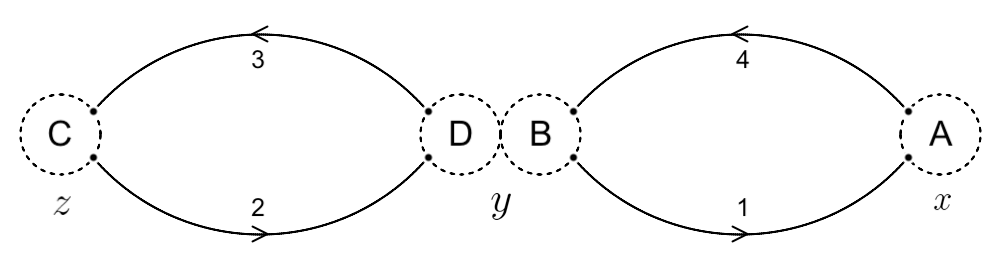
\includegraphics[width=0.45\textwidth]{../thesis-tex/imgs-MSc-thesis/Wick_stochastic_disc.png}
                  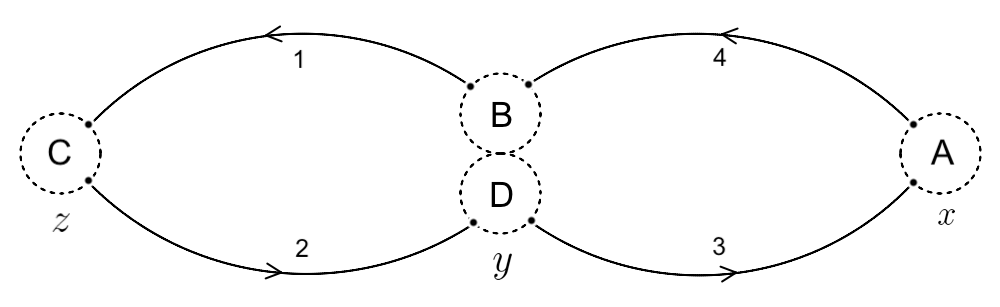
\includegraphics[width=0.4\textwidth]{../thesis-tex/imgs-MSc-thesis/Wick_stochastic_conn.png}
            \end{figure}
      \end{center}
      Two types of noise spinors contractions:
      \begin{equation*}
            \begin{gathered}
                  G_d =   \sum_{\vec y} \left\langle \left\langle \left(\gamma_5\xi^{(3,-)}_{1,A} (y) \right)^\dag \Gamma_B \zeta^{(4,+)}_1 (y) \cdot \left(\gamma_5\xi^{(1,-)}_{C,2} (y) \right)^\dag \Gamma_D \zeta^{(2,+)}_2 (y) \right\rangle^\text{noise} \right\rangle^{\text{sea}} \\
                  G_c = - \sum_{\vec y} \left\langle \left\langle \left(\gamma_5\xi^{(3,-)}_{1,A} (y) \right)^\dag \Gamma_D \zeta^{(2,+)}_2 (y) \cdot \left(\gamma_5\xi^{(1,-)}_{C,2} (y) \right)^\dag \Gamma_B \zeta^{(4,+)}_1 (y) \right\rangle^\text{noise} \right\rangle^{\text{sea}}
            \end{gathered}
      \end{equation*}
\end{frame}

\begin{frame}[noframenumbering]{$\star$ Lattice results: $\hat B_K$}
      \framesubtitle{\hspace*{1pt}}
      \begin{columns}
            \begin{column}{0.6\textwidth}
                  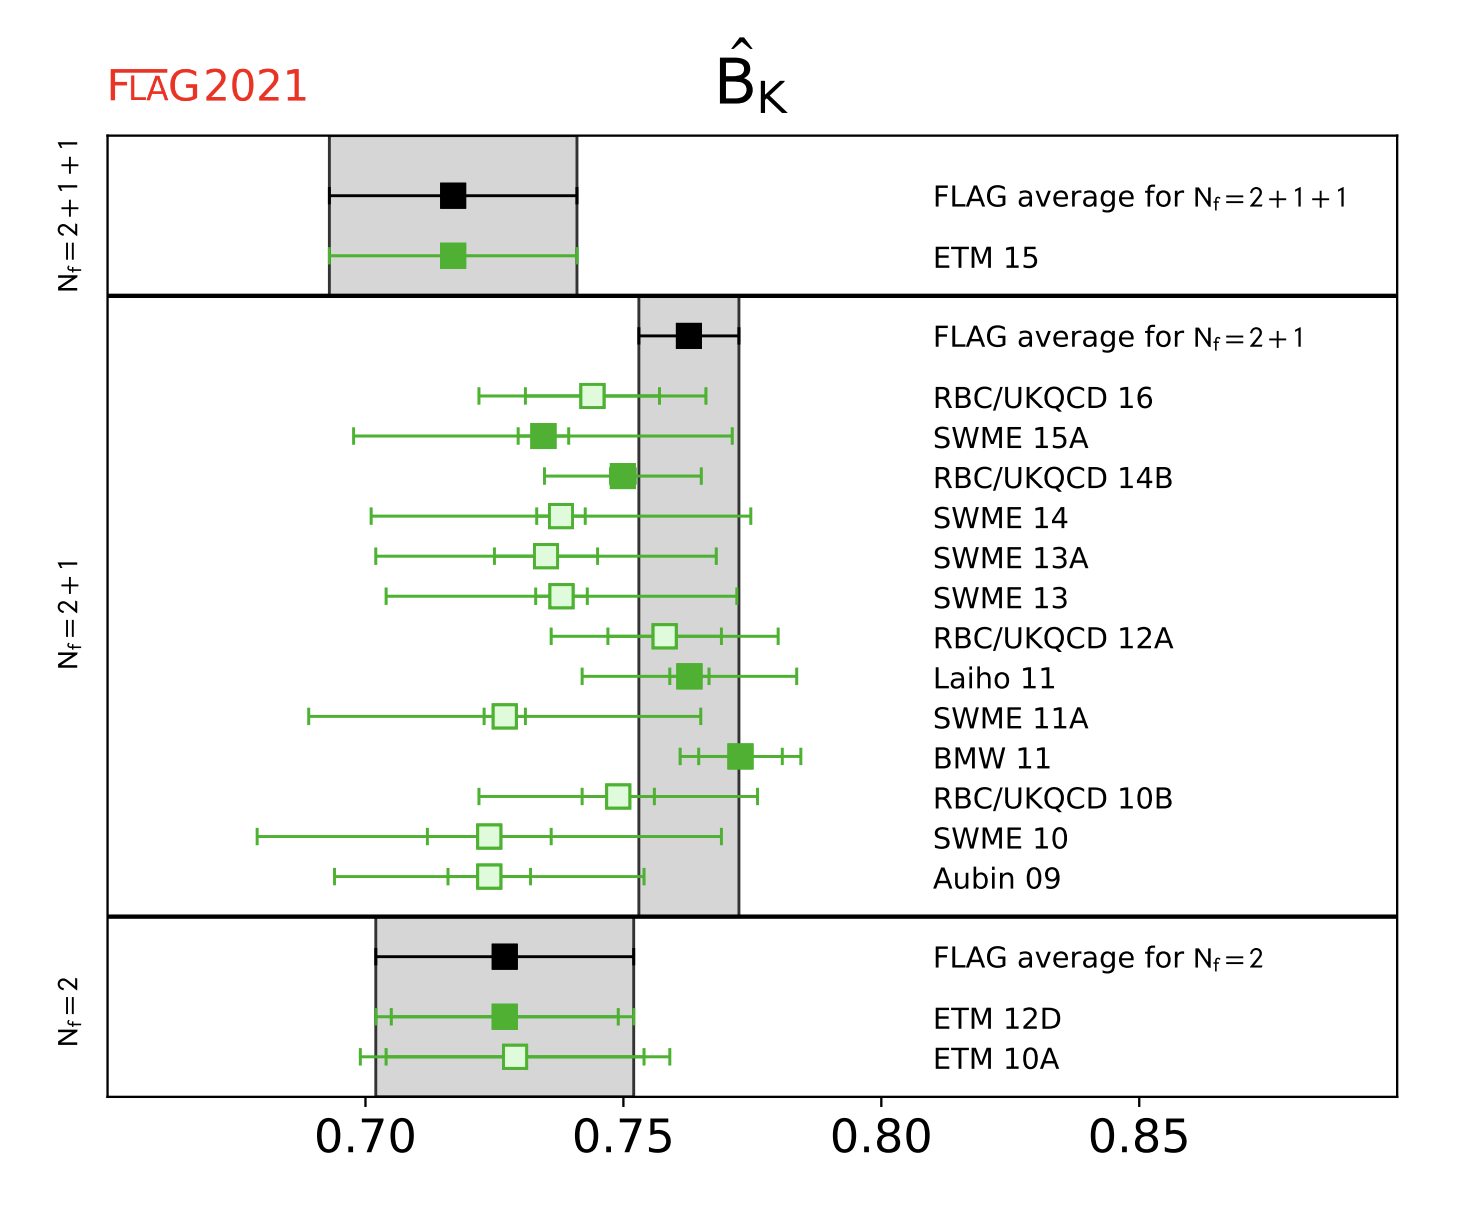
\includegraphics[width=\textwidth]{assets/hatBK-falg2021.png}
            \end{column}
            \begin{column}{0.4\textwidth}
                  Results for renormalization group invariant $\hat B_K$ $[6]$
                  \begin{itemize}
                        \item Different simulations use different regularizations
                        \item Results depend on both $B_K^\text{bare}$ and renormalisation
                        \item Strong deviation between simulations with different number of sea quarks
                  \end{itemize}
            \end{column}
      \end{columns}
\end{frame}

\begin{frame}[noframenumbering]{$\star$ Lattice results: $B_i, i \ge 2$}
      \framesubtitle{\hspace*{1pt}}
      \begin{columns}
            \begin{column}{0.75\textwidth}
                  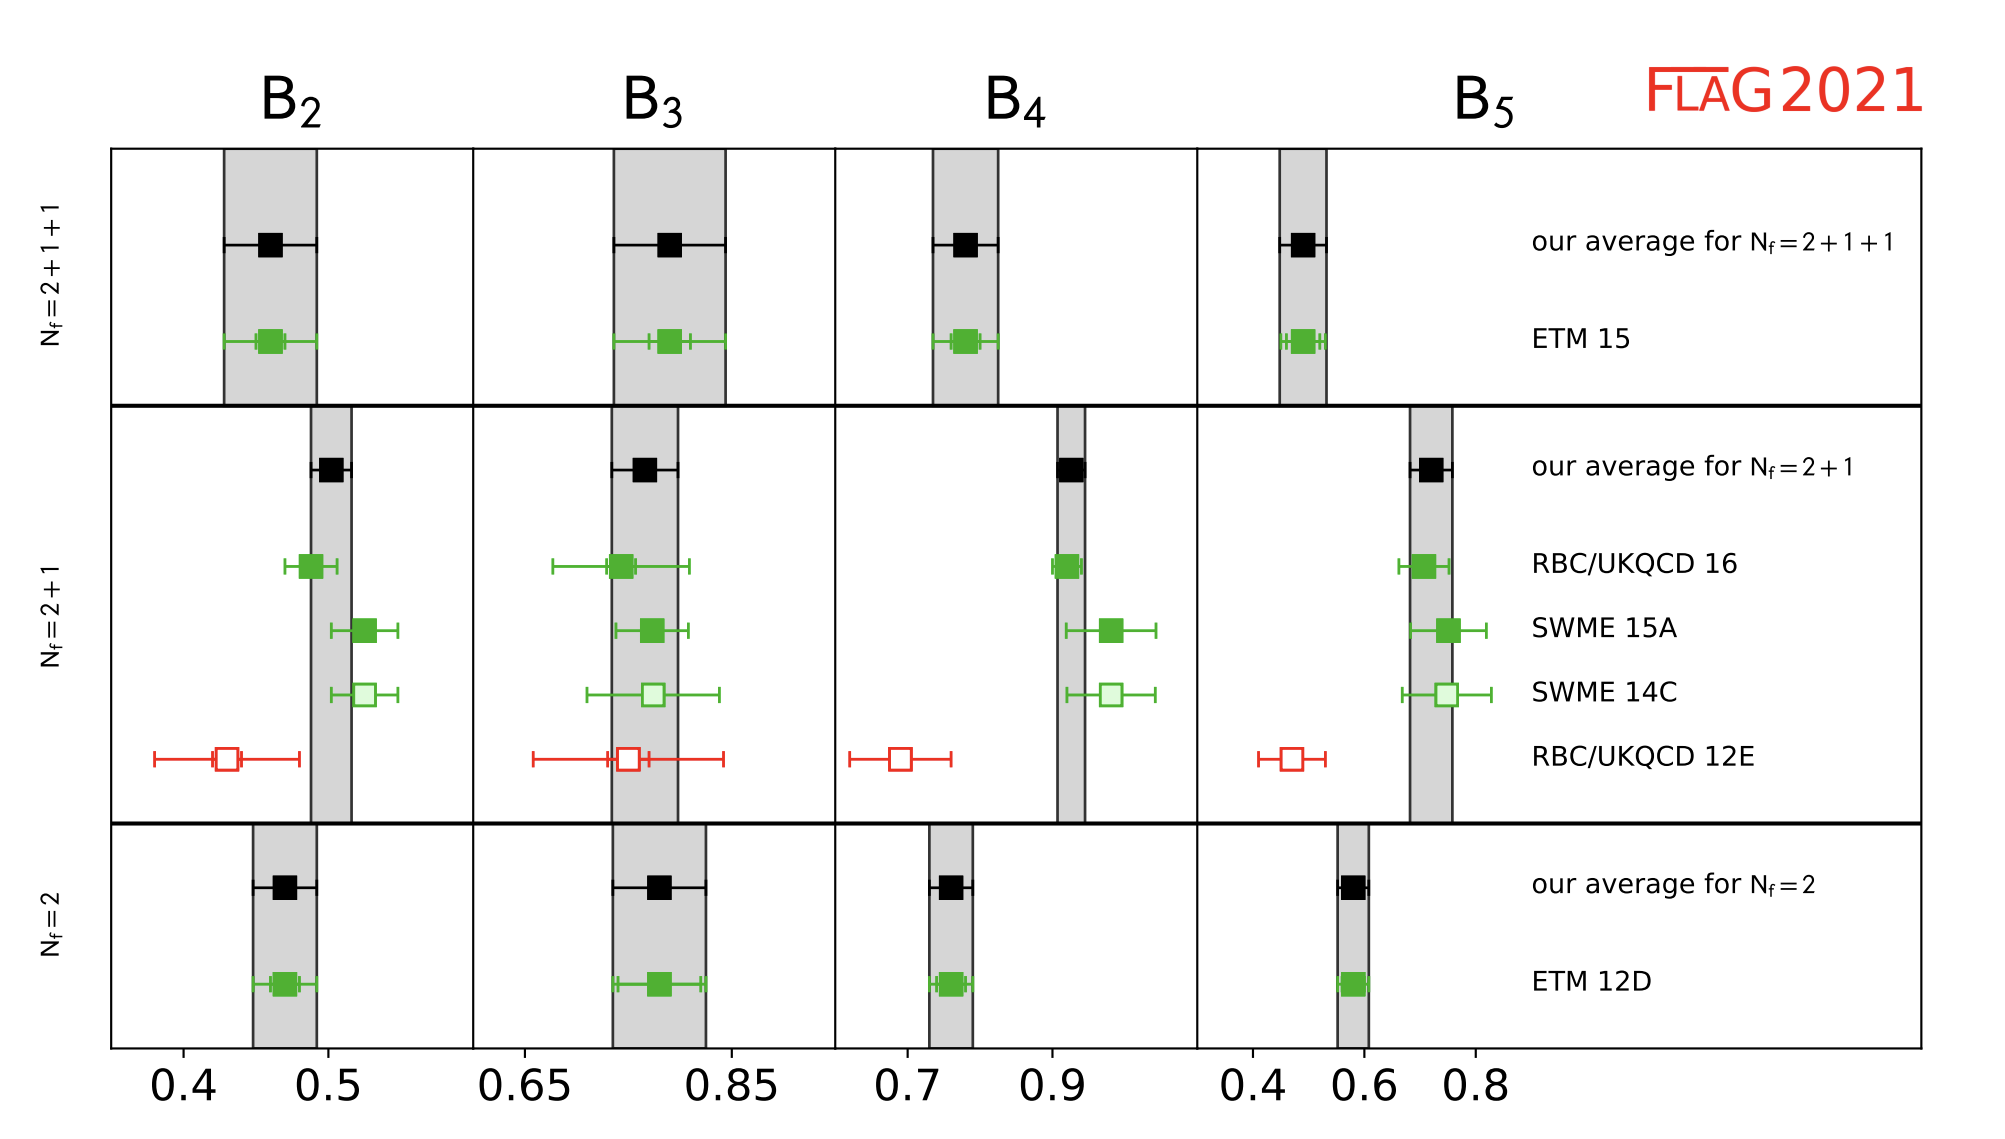
\includegraphics[width=\textwidth]{assets/Bi3GeV-falg2021.png}
            \end{column}
            \begin{column}{0.3\textwidth}
                  Results for renormalized bag parameters in $\overline{MS}$ scheme at $\mu = 3$ GeV
            \end{column}
      \end{columns}
\end{frame}

\end{document}
